\documentclass{article}
\usepackage[backend=biber,natbib=true,style=alphabetic,maxbibnames=50]{biblatex}
\addbibresource{/home/nqbh/reference/bib.bib}
\usepackage[utf8]{vietnam}
\usepackage{tocloft}
\renewcommand{\cftsecleader}{\cftdotfill{\cftdotsep}}
\usepackage[colorlinks=true,linkcolor=blue,urlcolor=red,citecolor=magenta]{hyperref}
\usepackage{amsmath,amssymb,amsthm,float,graphicx,mathtools,tikz}
\usepackage{enumitem}
\setlist{leftmargin=4mm}
\usetikzlibrary{angles,calc,intersections,matrix,patterns,quotes,shadings}
\allowdisplaybreaks
\newtheorem{assumption}{Assumption}
\newtheorem{baitoan}{}%{Bài toán}
\newtheorem{cauhoi}{Câu hỏi}
\newtheorem{conjecture}{Conjecture}
\newtheorem{corollary}{Corollary}
\newtheorem{dangtoan}{Dạng toán}
\newtheorem{definition}{Definition}
\newtheorem{dinhly}{Định lý}
\newtheorem{dinhnghia}{Định nghĩa}
\newtheorem{example}{Example}
\newtheorem{ghichu}{Ghi chú}
\newtheorem{hequa}{Hệ quả}
\newtheorem{hypothesis}{Hypothesis}
\newtheorem{lemma}{Lemma}
\newtheorem{luuy}{Lưu ý}
\newtheorem{nhanxet}{Nhận xét}
\newtheorem{notation}{Notation}
\newtheorem{note}{Note}
\newtheorem{principle}{Principle}
\newtheorem{problem}{Problem}
\newtheorem{proposition}{Proposition}
\newtheorem{question}{Question}
\newtheorem{remark}{Remark}
\newtheorem{theorem}{Theorem}
\newtheorem{vidu}{Ví dụ}
\usepackage[left=1cm,right=1cm,top=5mm,bottom=5mm,footskip=4mm]{geometry}
\def\labelitemii{$\circ$}
\DeclareRobustCommand{\divby}{%
	\mathrel{\vbox{\baselineskip.65ex\lineskiplimit0pt\hbox{.}\hbox{.}\hbox{.}}}%
}

\title{Problem: Root -- Bài Tập: Căn Thức}
\author{Nguyễn Quản Bá Hồng\footnote{Independent Researcher, Ben Tre City, Vietnam\\e-mail: \texttt{nguyenquanbahong@gmail.com}; website: \url{https://nqbh.github.io}.}}
\date{\today}

\begin{document}
\maketitle
\begin{abstract}
	Last updated version: \href{https://github.com/NQBH/elementary_STEM_beyond/blob/main/elementary_mathematics/grade_9/circle/problem/NQBH_circle_problem.pdf}{GitHub{\tt/}NQBH{\tt/}elementary STEM \& beyond{\tt/}elementary mathematics{\tt/}grade 9{\tt/}circle{\tt/}problem: set $\mathbb{Q}$ of circles [pdf]}.\footnote{\textsc{url}: \url{https://github.com/NQBH/elementary_STEM_beyond/blob/main/elementary_mathematics/grade_9/circle/problem/NQBH_circle_problem.pdf}.} [\href{https://github.com/NQBH/elementary_STEM_beyond/blob/main/elementary_mathematics/grade_9/circle/problem/NQBH_circle_problem.tex}{\TeX}]\footnote{\textsc{url}: \url{https://github.com/NQBH/elementary_STEM_beyond/blob/main/elementary_mathematics/grade_9/rational/problem/NQBH_circle_problem.tex}.}. 
\end{abstract}
\tableofcontents

%------------------------------------------------------------------------------%

\section{Bất Phương Trình}
Ta xét các dạng bất đẳng thức \& bất phương trình được sử dụng nhiều để tìm điều kiện xác định (ĐKXĐ) của căn thức bậc 2 \& tổng quát hơn là căn thức bậc chẵn (căn thức bậc lẻ luôn xác định miễn là biểu thức dưới dấu căn có nghĩa, không nhất thiết phải không âm như căn bậc chẵn bắt buộc).

\subsection{Bất phương trình chứa ẩn trong dấu giá trị tuyệt đối}
Với $f:D\subset\mathbb{R}\to\mathbb{R}$, $x\mapsto f(x)$ là 1 hàm số biến $x$, có $\forall a\in\mathbb{R}$, $a > 0$:
\begin{equation*}
	\boxed{|f(x)| < a\Leftrightarrow -a < f(x) < a,\ |f(x)|\le a\Leftrightarrow -a\le f(x)\le a,\ |f(x)| > a\Leftrightarrow\left[\begin{split}
		f(x) &< -a,\\
		f(x) &> a,
	\end{split}\right.,\ |f(x)| > a\Leftrightarrow\left[\begin{split}
	f(x) &\le -a,\\
	f(x) &\ge a.
	\end{split}\right.}
\end{equation*}
Để giải bất phương trình tích, ta thường sử dụng:

\begin{dinhly}[Dấu của nhị thức bậc nhất $ax + b$]
	Nhị thức $ax + b$, $a,b\in\mathbb{R}$, $a\ne0$, cùng dấu với $a$ với mọi giá trị của $x$ lớn hơn nghiệm của nhị thức (i.e., $a(ax + b) > 0$, $\forall x > -\frac{b}{a}$), trái dấu với $a$ với mọi giá trị của $x$ nhỏ hơn nghiệm của nhị thức (i.e., $a(ax + b) < 0$, $\forall x < -\frac{b}{a}$).
\end{dinhly}

\begin{baitoan}[\cite{Binh_Toan_9_tap_1}, Ví dụ 1, p. 5]
	Giải bất phương trình bậc 2: (a) $x^2 - 4x - 5 < 0$. (b) $x^2 - 2x - 1 > 0$. (c) $2x^2 - 6x + 5 > 0$.
\end{baitoan}

\begin{baitoan}[\cite{Binh_Toan_9_tap_1}, 1., p. 6]
	Giải bất phương trình bậc 2: (a) $x^2 - 4x - 21 > 0$. (b) $x^2 - 4x + 1 < 0$. (c) $3x^2 - x + 1 > 0$. (d) $2x^2 - 5x + 4 < 0$.
\end{baitoan}

\begin{baitoan}[Giải bất phương trình bậc nhất tổng quát]
	Giải \& biện luận theo $a,b,c\in\mathbb{R}$, $a\ne0$, bất phương trình: (a) $ax + b > 0$. (b) $ax + b < 0$. (c) $ax + b\le0$. (d) $ax + b\ge0$.
\end{baitoan}

\begin{baitoan}[Giải bất phương trình bậc nhất chứa trị tuyệt đối dạng tổng quát]
	Giải \& biện luận theo $a,b,c\in\mathbb{R}$, $a\ne0$, bất phương trình: (a) $|ax + b| > c$. (b) $|ax + b| < c$. (c) $|ax + b|\le c$. (d) $|ax + b|\ge c$.
\end{baitoan}

\begin{baitoan}[Giải bất phương trình bậc 2 tổng quát]
	Giải \& biện luận theo $a,b,c,d\in\mathbb{R}$, $a\ne0$, bất phương trình: (a) $ax^2 + bx + c > 0$. (b) $ax^2 + bx + c < 0$. (c) $ax^2 + bx + c\le0$. (d) $ax^2 + bx + c\ge0$.
\end{baitoan}

\begin{baitoan}[Giải bất phương trình bậc 2 chứa trị tuyệt đối dạng tổng quát]
	Giải \& biện luận theo $a,b,c,d\in\mathbb{R}$, $a\ne0$, bất phương trình: (a) $|ax^2 + bx + c| > d$. (b) $|ax^2 + bx + c| < d$. (c) $|ax^2 + bx + c|\le d$. (d) $|ax^2 + bx + c|\ge d$.
\end{baitoan}

\begin{baitoan}[Giải bất phương trình dạng tích tổng quát]
	Giải \& biện luận theo $a,x_i\in\mathbb{R}$, $\forall i = 1,2,\ldots,n$, với $n\in\mathbb{N}$, $a\ne0$, bất phương trình: (a) {\rm Bất phương trình bậc nhất dạng tích tổng quát:} $a(x - x_0) > 0$, $a(x - x_0) < 0$, $a(x - x_0)\le0$, $a(x - x_0)\ge0$. (b) {\rm Bất phương trình bậc 2 dạng tích tổng quát:} Với $x_1\le x_2$, $a(x - x_1)(x - x_2) > 0$, $a(x - x_1)(x - x_2) < 0$, $a(x - x_1)(x - x_2)\le0$, $a(x - x_1)(x - x_2)\ge0$. (c) {\rm Bất phương trình bậc 3 dạng tích tổng quát:} Với $x_1\le x_2\le x_3$, $a(x - x_1)(x - x_2)(x - x_3) > 0$, $a(x - x_1)(x - x_2)(x - x_3) < 0$, $a(x - x_1)(x - x_2)(x - x_3)\le0$, $a(x - x_1)(x - x_2)(x - x_3)\ge0$. (d) {\rm Bất phương trình bậc 4 dạng tích tổng quát:} Với $x_1\le x_2\le x_3\le x_4$, $a(x - x_1)(x - x_2)(x - x_3)(x - x_4) > 0$, $a(x - x_1)(x - x_2)(x - x_3)(x - x_4) < 0$, $a(x - x_1)(x - x_2)(x - x_3)(x - x_4)\le0$, $a(x - x_1)(x - x_2)(x - x_3)(x - x_4)\ge0$. (e${}^\star$) {\rm Bất phương trình bậc $n\in\mathbb{N}^\star$ dạng tích tổng quát:} Với $x_1\le x_2\le\cdots\le x_{n-1}\le x_n$, $a\prod_{i=1}^n (x - x_i) > 0$, $a\prod_{i=1}^n (x - x_i) < 0$, $a\prod_{i=1}^n (x - x_i)\le0$, $a\prod_{i=1}^n (x - x_i)\ge0$, trong đó sử dụng ký hiệu tích $\prod_{i=1}^n (x - x_i) = (x - x_1)(x - x_2)\cdots(x - x_n)$.
\end{baitoan}

\begin{baitoan}[Programming: Solve general inequations of product-form]
	Viết chương trình {\sf Pascal, Python, C{\tt/}C++} để giải các bất phương trình $P(x) > 0$, $P(x) < 0$, $P(x)\le0$, $P(x)\ge0$, với $P(x)\coloneqq a\prod_{i=1}^n (x - x_i) = a(x - x_1)(x - x_2)\cdots(x - x_n)$, trong đó $n\in\mathbb{N}^\star$, $a\in\mathbb{R}$, $a\ne0$, $x_i\in\mathbb{R}$, $\forall i = 1,2,\ldots,n$.
	\begin{itemize}
		\item {\sf Input.} Dòng 1: Số bộ test. Dòng 2: $n\in\mathbb{N}$, $a\in\mathbb{R}^\star$. Dòng 3: $n$ số thực không nhất thiết phân biệt chưa được sắp xếp thứ tự: $x_1,x_2,\ldots,x_n$. 
		\item {\sf Output.} 4 tập nghiệm của 4 bất phương trình $P(x) > 0$, $P(x) < 0$, $P(x)\le0$, $P(x)\ge0$.
		\item {\sf Sample.}
		\begin{table}[H]
			\centering\tt
			\begin{tabular}{|l|l|}
				\hline
				\verb|polynomial_inequation.inp| & \verb|polynomial_inequation.out| \\
				\hline
				2 & P(x) > 0: x < 2 \\
				1 -1.5 & P(x) < 0: x > 2 \\
				2 & P(x) <= 0: x >= 2 \\
				2 100 & P(x) >= 0: x <= 2 \\
				3 -4 & \\
				& P(x) > 0: x < -4 or x > 3 \\
				& P(x) < 0: -4 < x < 3 \\
				& P(x) <= 0: -4 <= x <= 3 \\
				& P(x) >= 0: x <= -4 or x => 3 \\
				\hline
			\end{tabular}
		\end{table}
	\end{itemize}
\end{baitoan}

%------------------------------------------------------------------------------%

\section{Căn Bậc 2 \& Số Vô Tỷ}
Ở Toán 7 (xem, e.g., \cite[\S5, pp. 27--29]{SGK_Toan_7_Canh_Dieu_tap_1}), ta đã biết dạng biểu diễn thập phân của số hữu tỷ là hữu hạn hoặc vô hạn tuần hoàn, dạng biểu diễn thập phân của số vô tỷ là vô hạn không tuần hoàn. Số hữu tỷ $a\in\mathbb{Q}$ nào cũng viết được dưới dạng $a = \dfrac{m}{n}$ với $m\in\mathbb{Z}$, $n\in\mathbb{N}^\star$.

\begin{baitoan}
	Chứng minh tổng, hiệu, tích, thương của 2 số hữu tỷ (số chia $\ne0$) là 1 số hữu tỷ.
\end{baitoan}

\begin{proof}[Chứng minh]
	Gọi 2 số hữu tỷ bất kỳ là $\dfrac{a}{b}$ \& $\dfrac{c}{d}$ với $a,b,c,d\in\mathbb{Z}$, $bd\ne0$. Tổng, hiệu, tích, thương của 2 số hữu tỷ (số chia $\ne0$) là 1 số hữu tỷ vì:
	\begin{align*}
		\frac{a}{b}\pm\frac{c}{d} = \frac{ad\pm bc}{bd},\ \frac{a}{b}\cdot\frac{c}{d} = \frac{ac}{bd},\ \forall a,b,c,d\in\mathbb{Z},\,bd\ne0; \frac{a}{b}:\frac{c}{d} = \frac{a}{b}\cdot\frac{d}{c} = \frac{ad}{bc},\ \forall a,b,c,d\in\mathbb{Z},\,bcd\ne0,
	\end{align*}
	trong đó điều kiện $bcd\ne0$ đã đảm bảo số chia khác 0.
\end{proof}

\begin{baitoan}[\cite{Binh_Toan_9_tap_1}, Ví dụ 2, p. 7]
	Chứng minh tổng \& hiệu của 1 số hữu tỷ với 1 số vô tỷ là 1 số vô tỷ.
\end{baitoan}

\begin{proof}[Giải]
	Chứng minh bằng phản chứng. Giả sử tồn tại 2 số $a\in\mathbb{Q}$ \& $b\in\mathbb{R}\backslash\mathbb{Q}$ sao cho $c = a + b\in\mathbb{Q}$. Ta có $b = c - a$, mà hiệu của 2 số hữu tỷ $c,a$ là 1 số hữu tỷ nên $b\in\mathbb{Q}$, mâu thuẫn với giả thiết, nên $c$ phải là số vô tỷ. Chứng minh tương tự cho hiệu.
\end{proof}

\begin{baitoan}
	(a) Chứng minh tích, \& thương của 1 số hữu tỷ khác $0$ với 1 số vô tỷ là 1 số vô tỷ.\footnote{Không cần yêu cầu số vô tỷ khác 0 vì 0 là số hữu tỷ nên hiển nhiên 1 số vô tỷ bất kỳ luôn khác 0.} (b) Chứng minh nếu tích hoặc thương của 1 số hữu tỷ với 1 số vô tỷ là 1 số hữu tỷ thì số hữu tỷ đó bằng $0$. 
\end{baitoan}

\begin{baitoan}
	Xét tính hữu tỷ, vô tỷ của 2 số $a,b\in\mathbb{R}$ thỏa mãn: (a) $a + b\in\mathbb{Q}$. (b) $a - b\in\mathbb{Q}$. (c) $ab\in\mathbb{Q}$. (d) $\dfrac{a}{b}\in\mathbb{Q}$. (e) $a^2 + b^2\in\mathbb{Q}$. (f) $a^2 - b^2\in\mathbb{Q}$. (g) $a^3 + b^3\in\mathbb{Q}$. (h) $a^3 - b^3\in\mathbb{Q}$. (i) $a^m + b^n\in\mathbb{Q}$ với $m,n\in\mathbb{N}^\star$. (j) $a^m - b^n\in\mathbb{Q}$ với $m,n\in\mathbb{N}^\star$.
\end{baitoan}

\begin{baitoan}[\cite{Binh_Toan_9_tap_1}, Ví dụ 3, p. 7]
	Xét xem 2 số $a,b$ có thể là số vô tỷ hay không, nếu: (a) $a + b$ \& $a - b$ là 2 số hữu tỷ. (b) $a - b$ \& $ab$ là 2 số hữu tỷ.
\end{baitoan}

\begin{baitoan}[\cite{Binh_Toan_9_tap_1}, Ví dụ 4, p. 7]
	Chứng minh: Nếu số tự nhiên $a$ không là số chính phương thì $\sqrt{a}$ là số vô tỷ.
\end{baitoan}

\begin{baitoan}[Mở rộng \cite{Binh_Toan_9_tap_1}, Ví dụ 4, p. 7]
	Chứng minh: Nếu số hữu tỷ $a$ không có dạng $\dfrac{m^2}{n^2}$ với $m,n\in\mathbb{N}$, $n\ne0$, thì $\sqrt{a}$ là số vô tỷ.
\end{baitoan}

\begin{baitoan}[\cite{Binh_Toan_9_tap_1}, 2., p. 8]
	Chứng minh các số sau là số vô tỷ: (a) $\sqrt{1 + \sqrt{2}}$. (b) $m + \dfrac{\sqrt{3}}{n}$ với $m,n\in\mathbb{Q}$, $n\ne0$.
\end{baitoan}

\begin{baitoan}[Mở rộng \cite{Binh_Toan_9_tap_1}, 2., p. 8]
	Cho $a,b,c\in\mathbb{Q}$. Tìm điều kiện của $a,b$ để: (a) $\sqrt{a + \sqrt{b}}\in\mathbb{Q}$. (b) $a + \dfrac{\sqrt{b}}{c}\in\mathbb{Q}$.
\end{baitoan}

\begin{baitoan}[\cite{Binh_Toan_9_tap_1}, 3., p. 8]
	Xét xem 2 số $a,b$ có thể là số vô tỷ hay không nếu: (a) $ab$ \& $\dfrac{a}{b}$ là các số hữu tỷ. (b) $a + b$ \& $\dfrac{a}{b}$ là các số hữu tỷ ($a + b\ne0$). (c) $a + b$, $a^2$, \& $b^2$ là các số hữu tỷ ($a + b\ne0$).
\end{baitoan}

\begin{baitoan}[\cite{Binh_Toan_9_tap_1}, 4., p. 8]
	So sánh 2 số: (a) $2\sqrt{3}$ \& $3\sqrt{2}$. (b) $6\sqrt{5}$ \& $5\sqrt{6}$. (c) $\sqrt{24} + \sqrt{45}$ \& $12$. (d) $\sqrt{37} - \sqrt{15}$ \& $2$.
\end{baitoan}

\begin{baitoan}[\cite{Binh_Toan_9_tap_1}, 5., p. 8]
	(a) Cho 1 ví dụ để chứng tỏ khẳng định $\sqrt{a}\le a$ với mọi số $a$ không âm là sai. (b) Cho $a > 0$. Với giá trị nào của $a$ thì $\sqrt{a} > a$?
\end{baitoan}

\begin{baitoan}[\cite{Binh_Toan_9_tap_1}, $\rm6^\star$., pp. 8--9]
	(a) Chỉ ra 1 số thực $x$ mà $x - \dfrac{1}{x}$ là số nguyên ($x\ne\pm1$). (b) Chứng minh nếu $x - \dfrac{1}{x}$ là số nguyên \& $x\ne\pm1$ thì $x$ \& $x + \dfrac{1}{x}$ là số vô tỷ. Khi đó $\left(x + \dfrac{1}{x}\right)^{2n}$ \& $\left(x + \dfrac{1}{x}\right)^{2n+1}$ là số hữu tỷ hay số vô tỷ?
\end{baitoan}

%------------------------------------------------------------------------------%

\section{Căn Thức Bậc 2 \& Hằng Đẳng Thức $\sqrt{A^2} = |A|$}

\begin{baitoan}[\cite{Binh_boi_duong_Toan_9_tap_1}, Ví dụ 1, p. 9]
	Trên 1 khúc sông, dòng chảy của nước ở bề mặt sông lớn hơn dòng chảy của nước ở đáy sông. Gọi $v$ {\rm km{\tt/}h} là vận tốc dòng chảy ở bề mặt sông, $f$ {\rm km{\tt/}h} là vận tốc dòng chảy ở đáy sông, các nhà vật lý (physicists) đã tính được $\sqrt{f} = \sqrt{v} - 1.3$. (a) Nếu vận tốc dòng chảy ở bề mặt sông là {\rm9 km{\tt/}h} thì vận tốc dòng chảy ở đáy sông là bao nhiêu? (b) Tính vận tốc dòng chảy ở bề mặt sông khi vận tốc dòng chảy ở đáy sông là {\rm20.25 km{\tt/}h}.
\end{baitoan}

\begin{baitoan}[\cite{Binh_boi_duong_Toan_9_tap_1}, Ví dụ 2, p. 9]
	Tìm $x\in\mathbb{R}$ thỏa: (a) $x^2 = 10$. (b) $\sqrt{2x + 1} = 5$. (c) $\sqrt{2x + 1} = \sqrt{3x - 1}$.
\end{baitoan}

\begin{baitoan}
	Giải \& biện luận phương trình theo các tham số $a,b,c,d\in\mathbb{R}$: (a) $x^2 = a$. (b) $\sqrt{ax + b} = c$. (c) $\sqrt{ax + b} = \sqrt{cx + d}$.
\end{baitoan}

\begin{baitoan}[\cite{Binh_boi_duong_Toan_9_tap_1}, Ví dụ 3, p. 10]
	So sánh: (a) $6$ \& $\sqrt{32}$. (b) $\sqrt{17} + \sqrt{10}$ \& $\sqrt{48}$. (c) $\sqrt{4 + \sqrt{5 + \sqrt{6}}}$ \& $3$.
\end{baitoan}

\begin{baitoan}[\cite{Binh_boi_duong_Toan_9_tap_1}, Ví dụ 4, p. 10]
	Rút gọn biểu thức: (a) $\sqrt{(a - 3)^2}$ với $a\le3$. (b) $2\sqrt{a^2 - 10a + 25}$ với $a\ge5$.
\end{baitoan}

\begin{baitoan}[\cite{Binh_boi_duong_Toan_9_tap_1}, Ví dụ 5, p. 10]
	Tìm $x\in\mathbb{R}$ thỏa: (a) $\sqrt{4x^2 - 28x + 49} = 7$. (b) $\sqrt{x - 10\sqrt{x} + 25} = 3$.
\end{baitoan}

\begin{baitoan}[\cite{Binh_boi_duong_Toan_9_tap_1}, Ví dụ 6, p. 11]
	Ngụy biện toán học: ``Bất kỳ 2 số nào cũng bằng nhau'': Với 2 số $a,b$ tùy ý, ta luôn có: $a^2 - 2ab + b^2 = b^2 - 2ba + a^2\Leftrightarrow(a - b)^2 = (b - a)^2$. Khai căn bậc 2 2 vế, ta được: $a - b = b - a$, suy ra $2a = 2b\Leftrightarrow a = b$. Vậy bất kỳ 2 số nào cũng bằng nhau. Tìm điểm sai.
\end{baitoan}

\begin{baitoan}[\cite{Binh_boi_duong_Toan_9_tap_1}, Ví dụ 7, p. 11]
	(a) Tìm {\rm GTNN} của biểu thức $A = \sqrt{x^2 - 8x + 20} - 12$. (b) Tìm {\rm GTLN} của biểu thức $B = 5 + \sqrt{-4x^2 - 4x + 6}$.
\end{baitoan}

\begin{luuy}
	(a) Để tìm {\rm GTNN} của 1 biểu thức $A$ có dạng $A = \sqrt{ax^2 + bx + c} + d$, ta cần biến đổi biểu thức dưới dấu căn của $A$ về dạng $f^2(x) + C$ ($C\ge0$ là hằng số) rồi nhận xét $\sqrt{f^2(x) + C}\ge\sqrt{C}$. Dấu ``$=$'' xảy ra $\Leftrightarrow f(x) = 0$. (b) Để tìm {\rm GTLN} của 1 biểu thức $B$ có dạng $B = \sqrt{ax^2 + bx + c} + d$, ta cần biến đổi biểu thức dưới dấu căn của $B$ về dạng $-f^2(x) + C$ ($C\ge0$  là hằng số) rồi nhận xét $\sqrt{-f^2(x) + C}\le\sqrt{C}$. Dấu ``$=$'' xảy ra $\Leftrightarrow f(x) = 0$.
\end{luuy}

\begin{baitoan}[\cite{Binh_boi_duong_Toan_9_tap_1}, 1.1., p. 12]
	Cho $\Delta ABC$ vuông tại $A$. Điền số thích hợp vào ô trống trong bảng:
	\begin{table}[H]
		\centering
		\begin{tabular}{|c|c|c|c|}
			\hline
			$AB$ & 7 cm & 0.3 m &  \\
			\hline
			$AC$ & 24 cm &  & 12 dm \\
			\hline
			$BC$ &  & 0.5 m & 15 dm \\
			\hline
		\end{tabular}
	\end{table}
\end{baitoan}

\begin{baitoan}[\cite{Binh_boi_duong_Toan_9_tap_1}, 1.2., p. 12]
	Tìm $x\in\mathbb{R}$ thỏa: (a) $3\sqrt{x + 1} = 18$. (b) $(2x)^2 = 64$. (c) $\sqrt{4x^2 - 4x + 1} = 7$.
\end{baitoan}

\begin{baitoan}[\cite{Binh_boi_duong_Toan_9_tap_1}, 1.3., p. 12]
	Tìm {\rm ĐKXĐ}: (a) $\sqrt{15 - 3x}$. (b) $\sqrt{\dfrac{x^2 + 1}{x - 1}}$. (c) $\sqrt{2x + 10} + \dfrac{1}{x^2 - 4}$.
\end{baitoan}

\begin{baitoan}[\cite{Binh_boi_duong_Toan_9_tap_1}, 1.4., p. 12]
	Tính: (a) $\sqrt{0.09}\cdot\sqrt{25} - \sqrt{49} + \sqrt{\dfrac{121}{100}}$. (b) $\sqrt{8^2 + 6^2} + 2\sqrt{\sqrt{625}}$.
\end{baitoan}

\begin{baitoan}[\cite{Binh_boi_duong_Toan_9_tap_1}, 1.5., p. 12]
	Cho 6 số: $\sqrt{21},5,\sqrt{38},-\sqrt{50},7,-\sqrt{37}$. Sắp xếp 6 số trên theo thứ tự tăng dần \& tìm số dương nhỏ nhất.
\end{baitoan}

\begin{baitoan}[\cite{Binh_boi_duong_Toan_9_tap_1}, 1.6., p. 12]
	Tính cạnh của hình vuông, biết diện tích của hình vuông đó bằng diện tích hình tam giác vuông có 2 cạnh góc vuông là {\rm12.8 m, 40 m}.
\end{baitoan}

\begin{baitoan}[\cite{Binh_boi_duong_Toan_9_tap_1}, 1.7., p. 12]
	Rút gọn biểu thức: (a) $\sqrt{(\sqrt{3} - 4)^2}$. (b) $\sqrt{6 - 2\sqrt{5}}$. (c) $\sqrt{4a^2} - 5a$ với $a > 0$. (d) $\sqrt{a^2 - 6a + 9} - 2\sqrt{a^2 + 8a + 16}$ với $-4\le a < 3$.
\end{baitoan}

\begin{baitoan}[\cite{Binh_boi_duong_Toan_9_tap_1}, 1.8., p. 12]
	Để tính giá trị của biểu thức $A = 3a + \sqrt{1 - 6a + 9a^2}$ tại $a = 2$, Việt làm như sau: $A = 3a + \sqrt{(1 - 3a)^2} = 3a + (1 - 3a) = 1$. Nam lại tính: $A = 3\cdot2 + \sqrt{1 - 6\cdot2 + 9\cdot2^2} = 6 + \sqrt{25} = 6 + 5 = 11$. Ai đúng ai sai? Sai ở đâu?
\end{baitoan}

\begin{baitoan}[\cite{Binh_boi_duong_Toan_9_tap_1}, 1.9., p. 12]
	Tìm $x\in\mathbb{R}$ thỏa: (a) $\sqrt{25x^2} = |-3|$. (b) $\sqrt{x^2 - 4x + 4} = \sqrt{x^2 + 4x + 4}$.
\end{baitoan}

\begin{baitoan}[\cite{Binh_boi_duong_Toan_9_tap_1}, 1.10., p. 12]
	Tìm {\rm GTLN} của biểu thức: (a) $A = \sqrt{7 - 2x^2}$. (b) $B = 7 + \sqrt{-4x^2 + 2x}$.
\end{baitoan}

\begin{baitoan}[\cite{Binh_boi_duong_Toan_9_tap_1}, 1.11., p. 13]
	Tìm {\rm GTNN} của biểu thức: (a) $A = 2\sqrt{x^2 + 3x + 5}$. (b) $B = \dfrac{3}{1 + \sqrt{2x - x^2 + 8}}$.
\end{baitoan}

\begin{baitoan}[\cite{Binh_boi_duong_Toan_9_tap_1}, 1.12., p. 13]
	Cho $a,b,c,d\in\mathbb{Q}$ thỏa $a + b + c + d = 0$. Chứng minh $\sqrt{(ab - cd)(bc - ad)(ca - bd)}\in\mathbb{Q}$.
\end{baitoan}

\begin{baitoan}[\cite{Binh_boi_duong_Toan_9_tap_1}, 1.13., p. 13]
	Cho hình vẽ:
	\begin{center}
		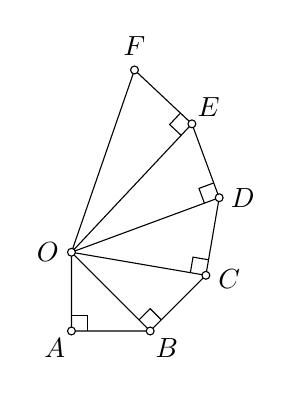
\begin{tikzpicture}
			\path
			(0,0) coordinate (A)
			(1,0) coordinate (B)
			(0,1) coordinate (O)
			($(B)!1cm!-90:(O)$) coordinate (C)
			($(C)!1cm!-90:(O)$) coordinate (D)
			($(D)!1cm!-90:(O)$) coordinate (E)
			($(E)!1cm!-90:(O)$) coordinate (F);
			\draw
			(O)--(A)--(B)--(C)--(D)--(E)--(F)--cycle (O)--(B) (O)--(C) (O)--(D) (O)--(E)
			pic[draw, angle radius=2mm]{right angle=O--A--B}
			pic[draw, angle radius=2mm]{right angle=O--B--C}
			pic[draw, angle radius=2mm]{right angle=O--C--D}
			pic[draw, angle radius=2mm]{right angle=O--D--E}
			pic[draw, angle radius=2mm]{right angle=O--E--F};
			\foreach \x/\g in {A/-135,B/-45,O/180,C/-10,D/0,E/45,F/90} \draw[fill=white] (\x) circle (.05) + (\g:.3) node{$\x$};
		\end{tikzpicture}
	\end{center}
	với $OA = AB = BC = CD = DE = È = 1$ {\rm cm}. (a) Tính độ dài 5 đoạn t hẳng $OB,OC,OD,OE,OF$. (b) Vẽ đoạn thẳng có độ dài $\sqrt{10}$ {\rm cm}. (c) Nêu cách vẽ đoạn thẳng có độ dài $\sqrt{n}$ {\rm cm} với $n\in\mathbb{N}$ bằng thước thẳng \& compa.
\end{baitoan}

\begin{baitoan}[\cite{Binh_boi_duong_Toan_9_tap_1}, 1.14., p. 13]
	Tìm $n\in\mathbb{N}$ sao cho $\sqrt{4n + 1}\in\mathbb{N}$.
\end{baitoan}

\begin{baitoan}[\cite{Binh_boi_duong_Toan_9_tap_1}, 1.15., p. 13]
	Cho $A = \sqrt{2 + \sqrt{2 + \cdots + \sqrt{2}}}$ gồm $2015$ dấu căn bậc 2. Chứng minh $A\notin\mathbb{N}$.
\end{baitoan}

%------------------------------------------------------------------------------%

\begin{baitoan}[\cite{Binh_Toan_9_tap_1}, Ví dụ 5, p. 7]
	Cho biểu thức $A = \sqrt{x - \sqrt{x^2 - 4x + 4}}$. (a) Tìm điều kiện xác định của biểu thức $A$. (b) Rút gọn biểu thức $A$.
\end{baitoan}

\begin{baitoan}[\cite{Binh_Toan_9_tap_1}, Ví dụ 6, p. 8]
	Tìm điều kiện xác định của các biểu thức: (a) $A = \dfrac{1}{\sqrt{x^2 - 2x - 1}}$. (b) $B = \dfrac{1}{\sqrt{x - \sqrt{2x + 1}}}$.
\end{baitoan}

\begin{baitoan}[\cite{Binh_Toan_9_tap_1}, Ví dụ 7, p. 8]
	Tìm các giá trị của $x$ sao cho $\sqrt{x + 1} < x + 3$.
\end{baitoan}

\begin{baitoan}[\cite{Binh_Toan_9_tap_1}, 7., p. 9]
	Tìm điều kiện xác định của các biểu thức: (a) $3 - \sqrt{1 - 16x^2}$. (b) $\dfrac{1}{1 - \sqrt{x^2 - 3}}$. (c) $\sqrt{8x - x^2 - 15}$. (d) $\dfrac{2}{\sqrt{x^2 - x + 1}}$. (e) $A = \dfrac{1}{\sqrt{x - \sqrt{2x - 1}}}$. (f) $B = \dfrac{\sqrt{16 - x^2}}{\sqrt{2x + 1}} + \sqrt{x^2 - 8x + 14}$.
\end{baitoan}

\begin{baitoan}[\cite{Binh_Toan_9_tap_1}, 8., p. 9]
	Cho biểu thức $A = \sqrt{x^2 - 6x + 9} - \sqrt{x^2 + 6x + 9}$. (a) Rút gọn biểu thức $A$. (b) Tìm các giá trị của $x$ để $A = 1$.
\end{baitoan}

\begin{baitoan}[\cite{Binh_Toan_9_tap_1}, 9., p. 9]
	Tìm các giá trị của $x$ sao cho: (a) $\sqrt{x^2 - 3}\le x^2 - 3$. (b) $\sqrt{x^2 - 6x + 9} > x - 6$.
\end{baitoan}

\begin{baitoan}[\cite{Binh_Toan_9_tap_1}, 10., p. 9]
	Cho $a + b + c = 0$ \& $abc\ne0$. Chứng minh hằng đẳng thức: $\sqrt{\dfrac{1}{a^2} + \dfrac{1}{b^2} + \dfrac{1}{c^2}} = \left|\dfrac{1}{a} + \dfrac{1}{b} + \dfrac{1}{c}\right|$.
\end{baitoan}

%------------------------------------------------------------------------------%

\section{$n$th Root -- Căn Bậc $n$}

%------------------------------------------------------------------------------%

\section{Miscellaneous}

%------------------------------------------------------------------------------%

\printbibliography[heading=bibintoc]

\end{document}